\documentclass[10pt]{article}
\usepackage[utf8]{inputenc}
\usepackage[italian]{babel}
\usepackage{multicol}
\usepackage[bookmarks]{hyperref}
\usepackage[a4paper, total={18cm, 25cm}]{geometry}
\usepackage{listings}
\usepackage{graphicx}
\usepackage{makecell}
\graphicspath{ {./img/} }
\usepackage{color}
\definecolor{mygray}{rgb}{0.5,0.5,0.5}
\usepackage{listings}
\usepackage{qtree}
\lstset{
	language=SQL,
	breaklines=true,
	keywordstyle=\bfseries,
	identifierstyle=\ttfamily,
	commentstyle=\color{mygray},
	morekeywords={database, REFERENCES, SCHEMA, AUTHORIZATION, PROCEDURE, WITH, CHECK, OPTION, FOR, EACH, ROW, DECLARE, BEFORE, AFTER, IF, TO, PRIVILEDGES, COMMIT, WORK, ROLLBACK, SORT},
}

\begin{document}
\renewcommand*\contentsname{Indice}
\title{Corso di Basi di Dati A.A. 2020/21\\Progetto "Fly Away"}
\author{Federico Matteoni\\Mat. 530257}
\date{08/01/2021}
\maketitle
\pagebreak
\section{Descrizione del dominio}
Il sistema si concentra sulla gestione dei biglietti, della loro prenotazione e vendita, sulla gestione delle promozioni e sulla gestione degli utenti.\\\\
Un utente può essere un agente di viaggio o un cliente. Un cliente può essere una società, con nome e partita iva, o un privato, con i dati anagrafici e il codice fiscale.\\
Un cliente può abbonarsi al programma fedeltà della compagnia, diventando infedele se non acquista biglietti per più di due anni.\\\\
Una prenotazione permette al cliente di prenotare non più di dieci biglietti su un singolo volo. Un cliente può avere più di una prenotazione attiva ma solo se tutte su voli diversi, e la prenotazione scade 3 giorni prima del volo.\\\\Un biglietto può essere legato ad una prenotazione o acquistato direttamente, e porta le indicazioni del volo e del cliente.\\\\
Un volo, con dati e orari di partenza e arrivo e informazioni sui posti disponibili, può avere una o più promozioni ad esso legate. Ogni volo assegna un quantitativo di punti agli utenti fedeli.\\\\Una promozione può essere legata ad un periodo di tempo o a determinati voli. Una prenotazione può essere aperta a tutti i clienti o essere esclusiva del programma Fedeltà, prevedendo uno sconto massimo del 25\% nel primo caso e del 50\% per i fedeli.
\section{Schema Concettuale}
\begin{center}
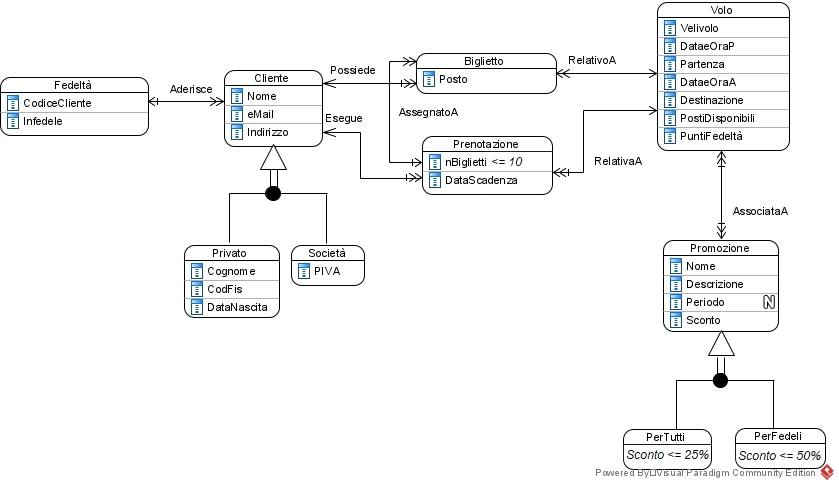
\includegraphics[scale=0.62]{Concettuale_FlyAway.jpg}
\end{center}
Il numero di righe nella tabella Biglietto legate alla medesima prenotazione non può essere superiore a 10.\\\\Ogni prenotazione assegnata al solito cliente deve essere legata ad un volo diverso.
\section{Schema Logico Relazionale}
\begin{center}
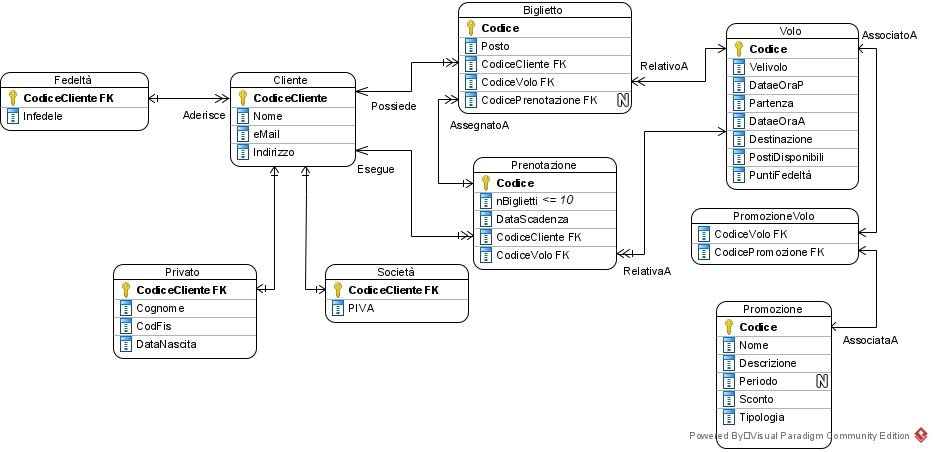
\includegraphics[scale=0.56]{LogicoRelazionale_FlyAway.jpg}
\end{center}
\begin{list}{}{}
	\item Fedeltà(\underline{CodiceCliente*}, Infedele)
	\item Cliente(\underline{CodiceCliente}, Nome, eMail, Indirizzo)
	\item Privato(\underline{CodiceCliente*}, Cognome, CodFis, DataNascita)
	\item Società(\underline{CodiceCliente*}, PIVA)
	\item Biglietto(\underline{Codice}, Posto, CodiceCliente*, CodiceVolo*, CodicePrenotazione*)
	\item Prenotazione(\underline{Codice}, nBiglietti, CodiceCliente*, CodiceVolo*)
	\item Volo(\underline{Codice}, Velivolo, DataeOraP, Partenza, DataeOraA, Destinazione, PostiDisponibili, PuntiFedeltà)
	\item PromozioneVolo(\underline{CodiceVolo*}, \underline{CodicePromozione*})
	\item Promozione(\underline{Codice}, Nome, Descrizione, Periodo, Sconto, Tipologia)
\end{list}
Tutte le dipendenze funzionali non banali presenti sono dipendenti da una chiave primaria. Un esempio, è la dipendenza \underline{CodiceCliente*} $\longrightarrow$ Cognome, nella relazione Privato: il \underline{CodiceCliente*} determina univocamente il campo Cognome, ma \underline{CodiceCliente*} è chiave primaria della relazione.\\\\
Una dipendenza funzionale che poteva essere presente è la seguente: se si aggiungesse un campo DataScadenza alla relazione Prenotazione, esso sarebbe univocamente determinato dal campo CodiceVolo*, che è chiave primaria della relazione Volo (in quanto la data di scadenza di una prenotazione in una istanza valida di Prenotazione è tre giorni prima del volo relativo), ma non è chiave della relazione Prenotazione.
\pagebreak
\section{Query SQL}
\begin{enumerate}
	\item Uso di proiezione, join e restrizione\\
	La lista di tutte le società che hanno prenotato almeno un biglietto nell'anno corrente.
	\begin{lstlisting}
	SELECT Nome, PIVA, eMail
	FROM Cliente
	JOIN Prenotazione ON Cliente.CodiceCliente = Prenotazione.CodiceCliente
	JOIN Volo ON Prenotazione.CodiceVolo = Volo.Codice
	JOIN Societa ON Cliente.CodiceCliente = Societa.CodiceCliente
	WHERE DataeOraP.YEAR = 2021
	\end{lstlisting}
	\item Uso di group by con having, where e sort\\
	La classifica degli utenti privati fedeli con più di N punti su voli negli ultimi 5 anni.
	\begin{lstlisting}
	SELECT Cognome, Nome, COUNT(PuntiFedelta) as Punti
	FROM Cliente
	JOIN Biglietto ON Cliente.CodiceCliente = Biglietto.CodiceCliente
	JOIN Volo ON Biglietto.CodiceVolo = Volo.Codice
	JOIN Fedelta ON Cliente.CodiceCliente = Fedelta.CodiceCliente
	JOIN Privato ON Cliente.CodiceCliente = Privato.CodiceCliente
	WHERE DataeOraP.YEAR >= 2016
	GROUP BY Cliente.CodiceCliente
	HAVING Punti > N
	ORDER BY Punti
	\end{lstlisting}
	\item Uso di join, group by con having e where\\
	La lista delle promozioni sui voli nel 2020 su più di 5 voli, specificando su quanti voli è stata applicata ogni promozione.
	\begin{lstlisting}
	SELECT Nome, COUNT(CodiceVolo) AS Voli
	FROM Promozione
	JOIN PromozioneVolo
		ON Promozione.Codice = PromozioneVolo.CodicePromozione
	JOIN Volo on PromozioneVolo.CodiceVolo = Volo.Codice
	WHERE Volo.DataeOraP.YEAR = 2020
	GROUP BY PromozioneVolo.CodicePromozione
	HAVING Voli > 5
	\end{lstlisting}
	\item Uso di select annidata con quantificazione esistenziale\\La lista delle promozioni su voli che assegnano meno di N punti fedeltà.
	\begin{lstlisting}
	SELECT Nome, Descrizione
	FROM Promozione
	JOIN PromozioneVolo
		ON Promozione.Codice = PromozioneVolo.CodicePromozione
	WHERE EXISTS	(SELECT Volo.Codice
			FROM Volo
			WHERE Volo.Codice = PromozioneVolo.CodiceVolo
			AND Volo.PuntiFedelta < N)
	\end{lstlisting}
	
	\item Uso di select annidata con quantificazione universale\\
	La lista delle promozioni su periodo.
	\begin{lstlisting}
	SELECT Nome, Descrizione
	FROM Promozione
	WHERE NOT EXISTS (SELECT *
		FROM PromozioneVolo
		WHERE Promozione.Codice = PromozioneVolo.CodicePromozione)
	\end{lstlisting}
	\pagebreak
	\item Uso di subquery di confronto quantificato usando una subquery\\
	La lista dei voli che forniscono più punti della media
	\begin{lstlisting}
	SELECT Partenza, Destinazione
	FROM Volo
	WHERE PuntiFedelta >	(SELECT AVG(PuntiFedelta)
				FROM Volo)
	\end{lstlisting}
	
\end{enumerate}
\section{Piani di accesso}
\begin{enumerate}
	\item Scrivere un piano di accesso logico delle query 1, 2 e 3
	\begin{list}{}{}
		\item[1.]		
\Tree [.$\Pi_{Nome, PIVA, eMail}$ [.$\sigma_{DataeOraP.YEAR=2021}$ [.$\bowtie$ [.$\bowtie_{CodiceVolo=Codice}$ [.$\bowtie$ Cliente Prenotazione ] Volo ] Società ] ] ]

		\item[2.]		
		\Tree [.$\tau_{Punti}$ [.$\Pi_{Cognome, Nome, Punti}$ [.$\sigma_{Punti > N}$ [.$\rho_{COUNT(PuntiFedelta)\leftarrow Punti}$ [.$_{CodiceCliente}\gamma_{COUNT(PuntiFedelta)}$ [.$\sigma_{DataeOraP.YEAR \geq 2016}$ [ .$\bowtie$ [.$\bowtie$ [.$\bowtie_{CodiceVolo=Codice}$ [.$\bowtie$ Cliente Biglietto ] Volo ] Fedeltà ] Privato ] ] ] ] ] ] ]
		\pagebreak
		\item[3.]		
		\Tree [.$\Pi_{Nome, Voli}$ [.$\sigma_{Voli>5}$ [.$\rho_{COUNT(CodiceVolo)\leftarrow Voli}$ [.$_{CodicePromozione}\gamma_{COUNT(CodiceVolo)}$ [.$\sigma_{DataeOraP.YEAR=2020}$ [.$\bowtie_{Volo.Codice=CodiceVolo}$ [.$\bowtie_{Promozione.Codice=CodicePromozione}$ Promozione PromozioneVolo ] Volo ] ] ] ] ] ]
	\end{list}
	\item Scrivere un piano di accesso fisico efficiente per i tre piani di accesso logico al punto 1 che non fanno uso di indici e (opzionale) verificare se la sort prima della group by può essere evitata\\1.\Tree [.Project(\{"Nome","PIVA","eMail"\}) [.NestedLoop("C.CodiceCliente=S.CodiceCliente") [.NestedLoop("P.CodiceVolo=V.Codice") [.NestedLoop("C.CodiceCliente=P.CodiceCliente") TableScan("Cliente") TableScan("Prenotazione") ] [.Filter("DataeOraP.YEAR=2021") TableScan("Volo") ] ] TableScan("Società") ] ]\\Per questioni di spazio, laddove possibile i nomi delle tabelle sono stati abbreviati con le loro iniziali.\\\\
	\pagebreak
	\begin{flushleft}
		2. In questo caso la Sort prima di GroupBy può essere evitata ordinando le tabelle sugli attributi di giunzione con SortMerge.\\\Tree [.Project(\{"Cognome,Nome,COUNT(PuntiFedeltà)"\}) [.Sort(\{"COUNT(PuntiFedeltà)"\}) [.Filter("COUNT(PuntiFedeltà$>$N") [.GroupBy\\(\{"CodiceCliente"\},\{"COUNT(PuntiFedeltà)"\}) [ .SortMerge\\("C.CodiceCliente=P.CodiceCliente") [.NestedLoop\\("C.CodiceCliente=F.CodiceCliente") [.NestedLoop\\("B.CodiceVolo=V.Codice") [.NestedLoop\\("C.CodiceCliente=B.CodiceCliente") TableScan\\("Cliente") TableScan\\("Biglietto") ] [.Filter\\("DataeOraP.YEAR$>=$2016") TableScan\\("Volo") ] ] TableScan\\("Fedeltà") ] TableScan\\("Privato") ] ] ] ] ]
	\end{flushleft}
		\pagebreak
	\begin{flushleft}
		3. Anche in questo caso la Sort prima di GroupBy può essere evitata ordinando le tabelle sugli attributi di giunzione con SortMerge.\\\Tree [.Project(\{"Nome,COUNT(CodiceVolo)"\} [.Filter("COUNT(CodiceVolo)$>$5") [.GroupBy(\{"CodicePromozione"\},\{"COUNT(CodiceVolo)"\}) [.NestedLoop("PV.CodiceVolo=V.Codice") [.SortMerge("P.Codice=PV.CodicePromozione") TableScan("Promozione") TableScan("PromozioneVolo") ] [.Filter("DataeOraP.YEAR=2020") TableScan("Volo") ] ] ] ] ]
	\end{flushleft}
	\item Scrivere un piano di accesso fisico efficiente per i tre piani di accesso logico al punto 1 che fanno uso di due indici (o comunque del numero massimo di indici possibili) e (opzionale) verificare se la sort prima della group by può essere evitata\\1.\Tree [.Project(\{"Nome","PIVA","eMail"\}) [.NestedLoop("C.CodiceCliente=S.CodiceCliente") [.NestedLoop("P.CodiceVolo=V.Codice") [.NestedLoop("C.CodiceCliente=P.CodiceCliente") TableScan("Cliente") TableScan("Prenotazione") ] IndexFilter\\("Volo","DataeOraP.YEAR=2021") ] IndexScan\\("Società",\\"C.CodiceCliente=\\S.CodiceCliente") ] ]\\Per questioni di spazio, laddove possibile i nomi delle tabelle sono stati abbreviati con le loro iniziali.\\\\
	\pagebreak
	\begin{flushleft}
		2. In questo caso la Sort prima di GroupBy può essere evitata ordinando le tabelle sugli attributi di giunzione con SortMerge.\\\Tree [.Project(\{"Cognome,Nome,COUNT(PuntiFedeltà)"\}) [.Sort(\{"COUNT(PuntiFedeltà)"\}) [.Filter("COUNT(PuntiFedeltà$>$N") [.GroupBy\\(\{"CodiceCliente"\},\{"COUNT(PuntiFedeltà)"\}) [ .SortMerge\\("C.CodiceCliente=P.CodiceCliente") [.NestedLoop\\("C.CodiceCliente=\\F.CodiceCliente") [.NestedLoop\\("B.CodiceVolo=V.Codice") [.NestedLoop\\("C.CodiceCliente=\\B.CodiceCliente") TableScan\\("Cliente") IndexScan\\("Biglietto",\\"C.CodiceCliente=\\B.CodiceCliente") ] IndexFilter\\("Volo",\\"DataeOraP.YEAR$>=$2016") ] IndexScan\\("Fedeltà",\\"C.CodiceCliente=\\F.CodiceCliente") ] IndexScan\\("Privato",\\"C.CodiceCliente=\\P.CodiceCliente") ] ] ] ] ]
	\end{flushleft}
		\pagebreak
	\begin{flushleft}
		3. Anche in questo caso la Sort prima di GroupBy può essere evitata ordinando le tabelle sugli attributi di giunzione con SortMerge.\\\Tree [.Project(\{"Nome,COUNT(CodiceVolo)"\} [.Filter("COUNT(CodiceVolo)$>$5") [.GroupBy(\{"CodicePromozione"\},\{"COUNT(CodiceVolo)"\}) [.NestedLoop("PV.CodiceVolo=V.Codice") [.SortMerge("P.Codice=PV.CodicePromozione") TableScan("Promozione") TableScan("PromozioneVolo") ] IndexFilter("Volo","DataeOraP.YEAR=2020") ] ] ] ]
	\end{flushleft}
\end{enumerate}
\end{document}